% ---------------------------------------------------------------------------- %
\begin{figure}
	\centering
	\subfigure[\label{fig:linguometer:technical:interference:isd2:1}]
	{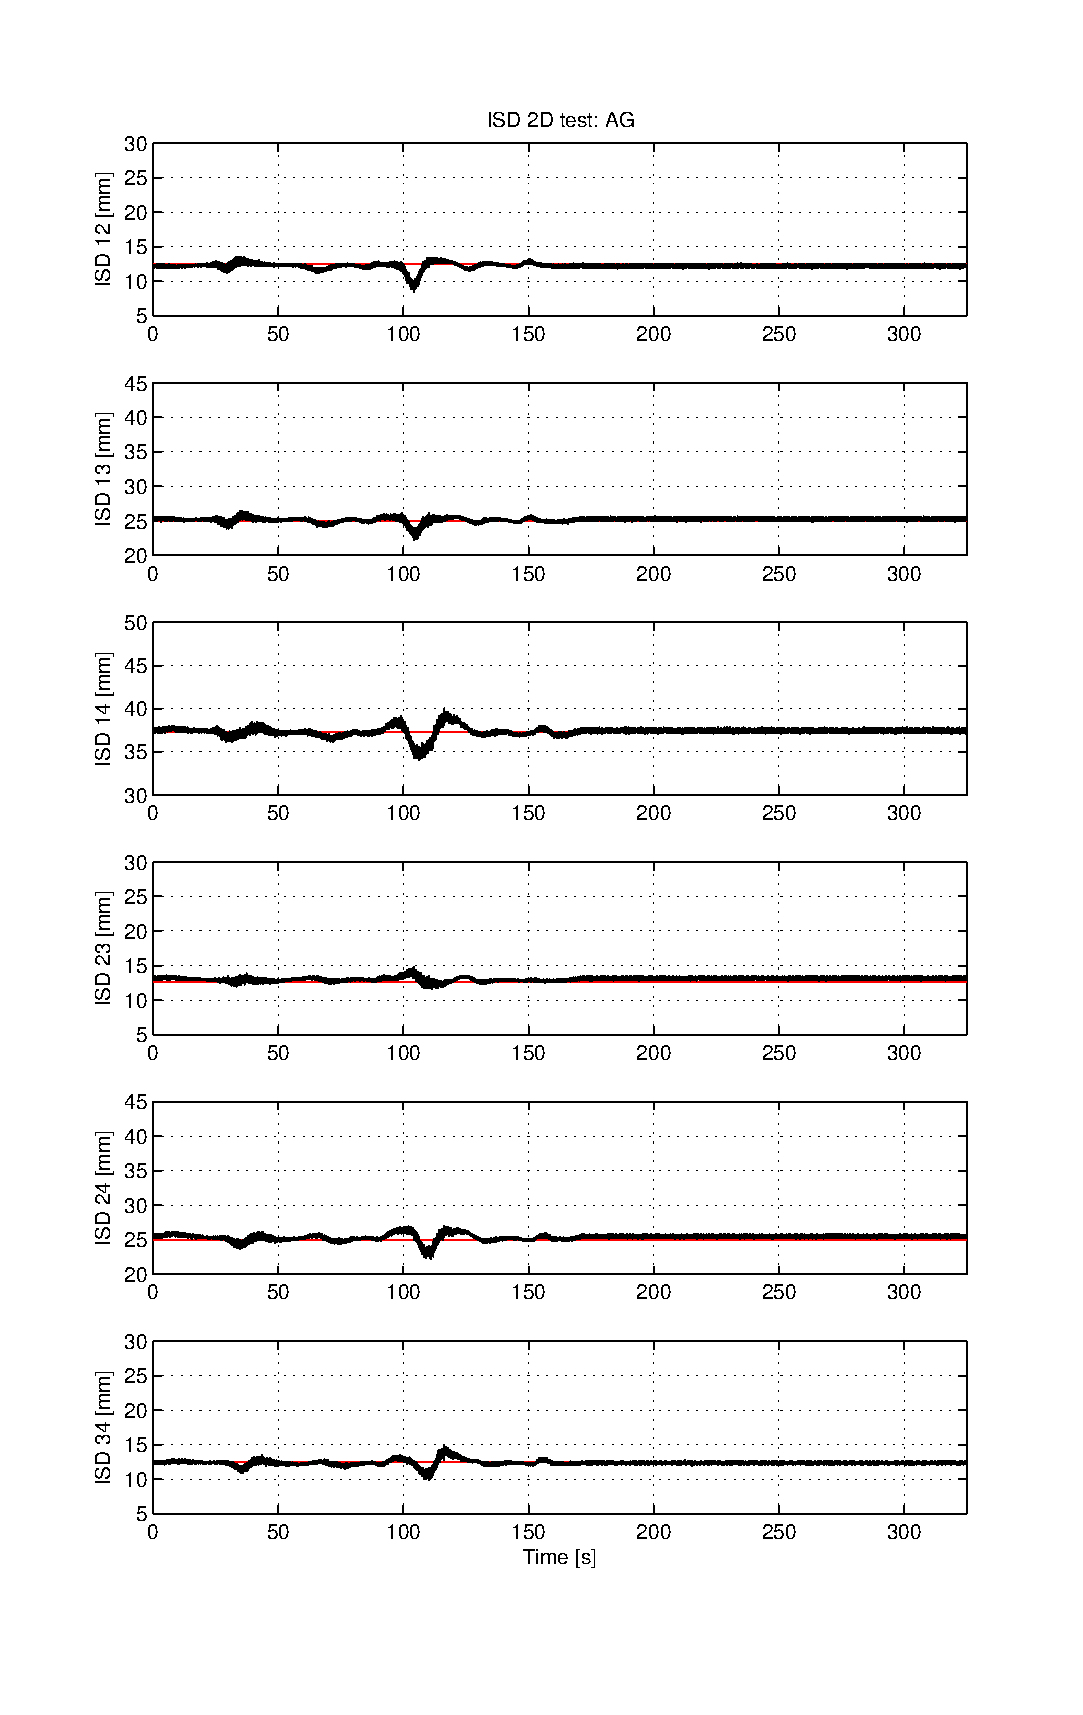
\includegraphics[width=0.35\textwidth]{include/linguometer/images/int_isd2d_1.eps}}
	\subfigure[\label{fig:linguometer:technical:interference:isd2:2}]
	{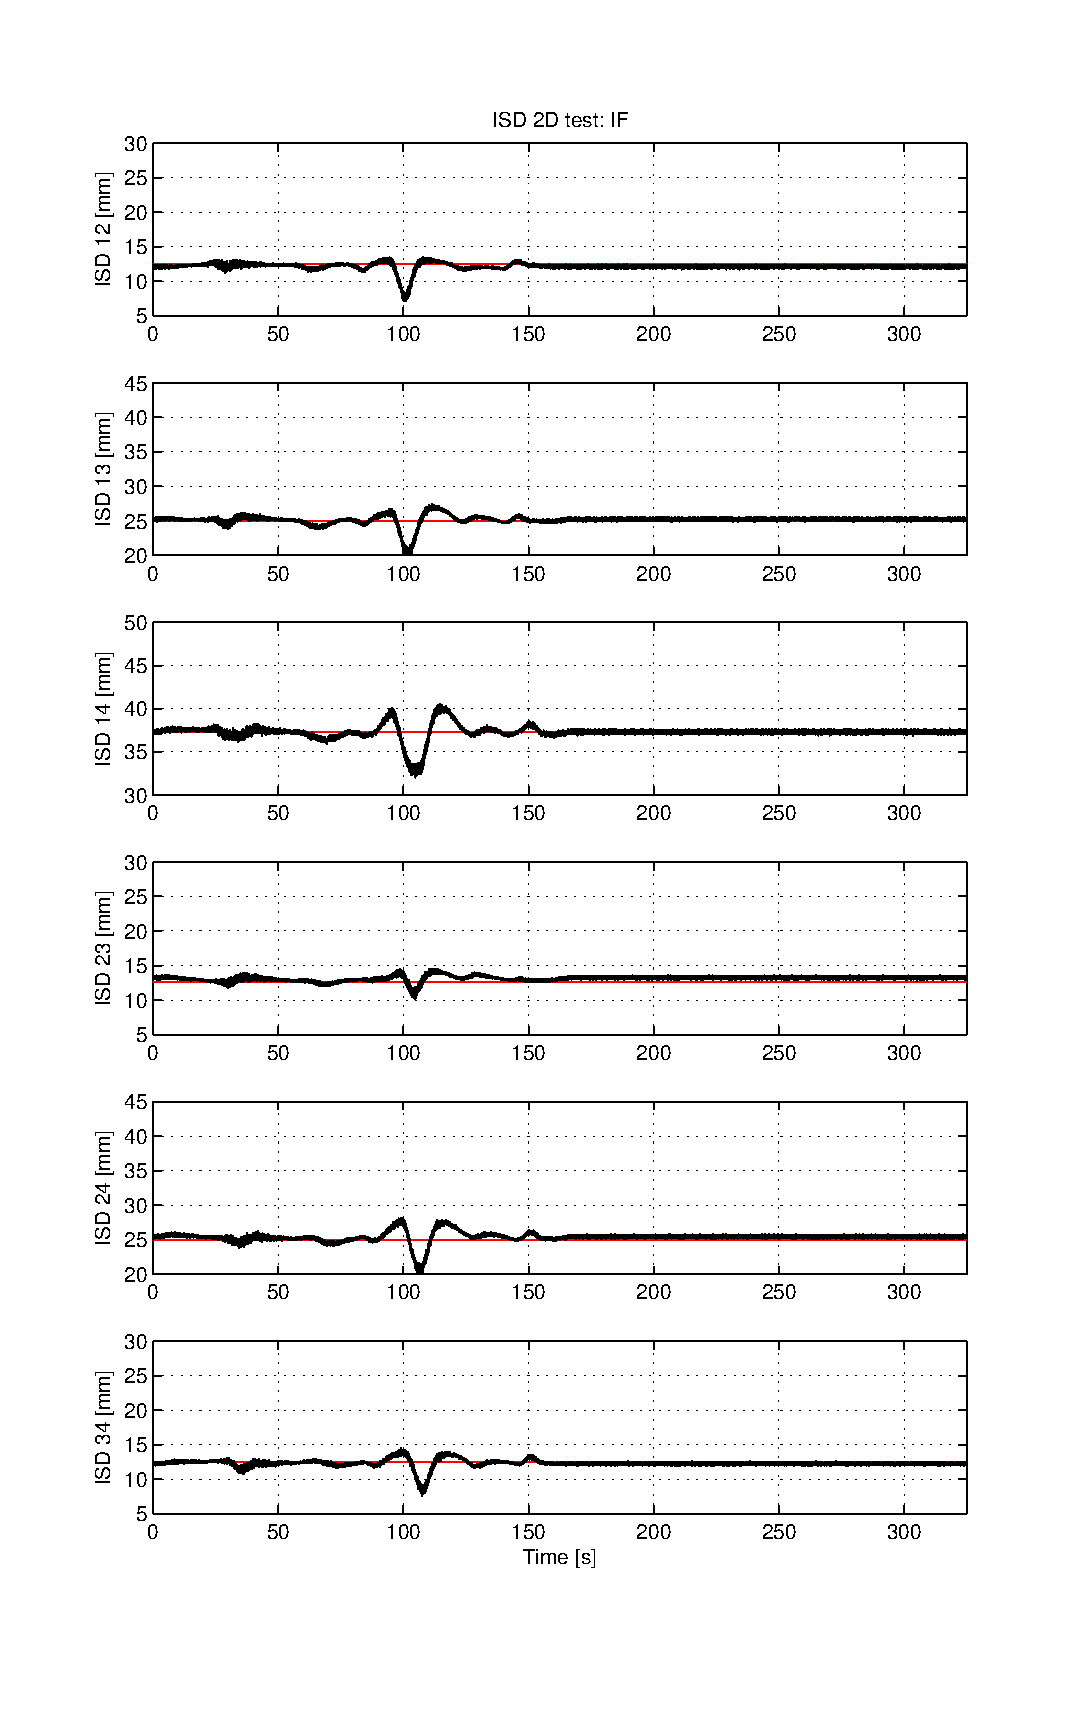
\includegraphics[width=0.35\textwidth]{include/linguometer/images/int_isd2d_2.eps}}

	\subfigure[\label{fig:linguometer:technical:interference:isd2:3}]
	{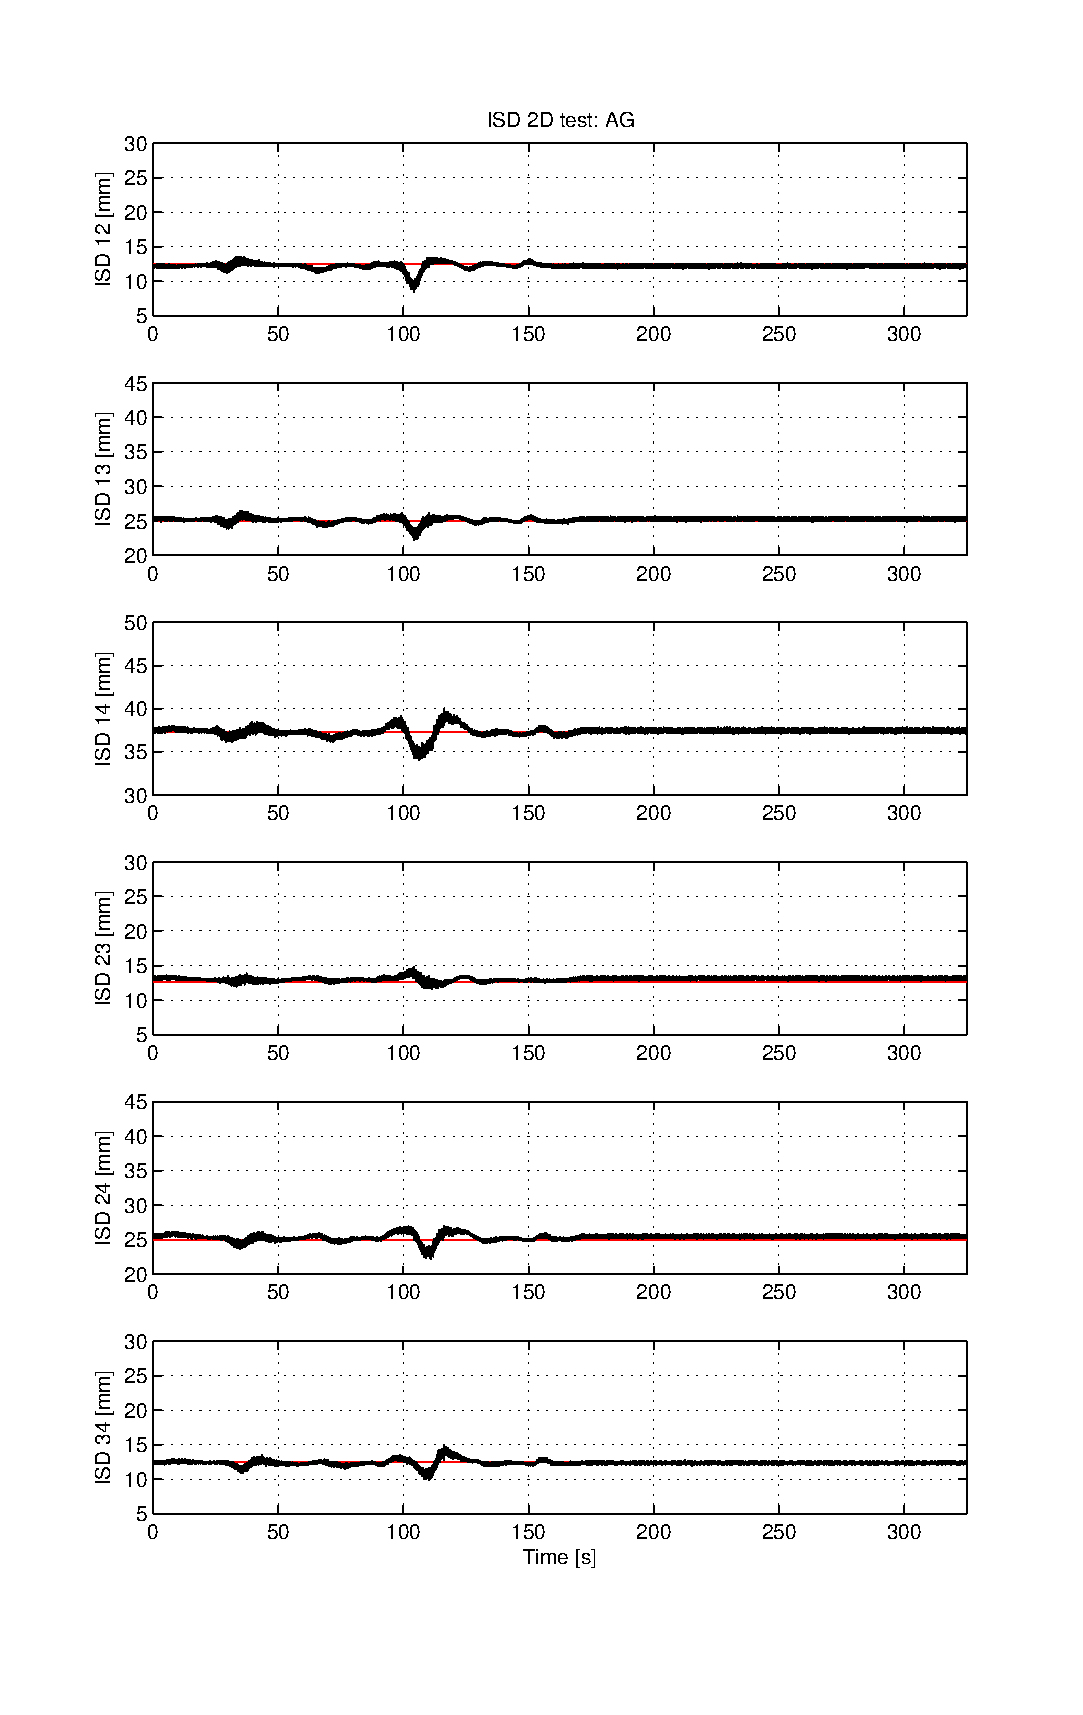
\includegraphics[width=0.35\textwidth]{include/linguometer/images/int_isd2d_3.eps}}
	\hspace{0.35\textwidth}
	
	\caption[ISD results (ad-hoc test, XY)]{\textbf{ISD results (ad-hoc test, XY)}:
	ISDs calculated considering the first two Cartesian coordinates of each 
	acquired sample (X and Y).
	(a) AG test, (b) IF test and (c) LM test.}
	\label{fig:linguometer:technical:interference:isd2}
\end{figure}
% ---------------------------------------------------------------------------- %
